\subsection{EXISTENCE OF APPROXIMATE SOLUTIONS}

Given a number \(\varepsilon > 0\) we shall say that a continuous map u of I into H is an approximate solution to within \(\varepsilon\) of the differential equation

\[
\mathbf {x} ^ {\prime} = \mathbf {f} (t, \mathbf {x})\tag{1}
\]

if, at all the points of the complement of a countable subset of I, the function u admits a derivative which satisfies the condition

\[
\left| \left| \mathbf {u} ^ {\prime} (t) - \mathbf {f} (t, \mathbf {u} (t)) \right| \right| \leqslant \varepsilon .\tag{7}
\]

Let \((t_{0}, \mathbf{x}_{0})\) be a point of \(I \times H\) ; since f satisfies the hypotheses of lemma 1 (IV, p.~165) there exist a compact neighbourhood J of \(t_{0}\) in I such that \(\mathbf{f}(t, \mathbf{x}_{0})\) is bounded on J, and an open ball S with centre \(\mathbf{x}_{0}\) contained in H, such that \(\mathbf{f}(t, \mathbf{x}) - \mathbf{f}(t, \mathbf{x}_{0})\) is bounded on \(J \times S\) ; it follows that \(\mathbf{f}(t, \mathbf{x})\) is bounded on \(J \times S\) . Throughout this subsection J will denote a compact interval which is a neighbourhood of \(t_{0}\) in I, S will be an open ball with centre \(\mathbf{x}_{0}\) and radius r contained in H, with J and S such that f is bounded on \(J \times S\) ; and M will denote the supremum of \(\| \mathbf{f}(t, \mathbf{x}) \|\) over \(J \times S\) .

PROPOSITION 3. On every compact interval with left (or right) endpoint \(t_{0}\) contained in J, with length less than \(r/(M + \varepsilon)\) , there exists an approximate solution to within \(\varepsilon\) of equation (1), with values in S, and equal to \(x_{0}\) at \(t_{0}\) .

We suppose that \(t_{0}\) is not the right-hand endpoint of J, and prove the proposition for intervals with left-hand endpoint \(t_{0}\) . Let M be the set of solutions of (1) to within \(\varepsilon\) , each of which takes values in S, is equal to \(x_{0}\) at \(t_{0}\) , and is defined on a half open interval \([t_{0}, b[\) contained in J (the interval depending on the approximate solution under consideration). First we show that M is not empty. Let c be right limit of \(\mathbf{f}(t, \mathbf{x}_{0})\) at \(t_{0}\) ; by lemma 1 (IV, p.~165) the function \(\mathbf{f}\big(t, \mathbf{x}_{0} + \mathbf{c}(t - t_{0})\big)\) has a right limit equal to c at \(t_{0}\) , so the restriction of the function \(\mathbf{x}_{0} + \mathbf{c}(t - t_{0})\) to a sufficiently small half open interval \([t_{0}, b[\) will belong to M.

We order the set M by the relation ``u is a restriction of v'', and show that M is inductive (Set Theory, III, p.~154). Let \((\mathbf{u}_{\alpha})\) be a totally ordered subset of M and \([t_{0}, b_{\alpha}[\) the interval where \(u_{\alpha}\) is defined: for \(b_{\alpha} \leqslant b_{\beta}\) the function \(u_{\beta}\) is thus an extension of \(u_{\alpha}\) . The union of the intervals \([t_{0}, b_{\alpha}[\) is an interval \([t_{0}, b[\) contained in J, and there exists one and only one function u defined on \([t_{0}, b[\) that coincides with \(u_{\alpha}\) on \([t_{0}, b_{\alpha}[\) for each \(\alpha\) ; among the \(b_{\alpha}\) there is an increasing sequence \((b_{\alpha_{n}})\) tending to b; since u agrees with \(u_{\alpha_{n}}\) on \([t_{0}, b_{\alpha_{n}}[\) the function u admits a derivative satisfying (7) at all the points of the complement of a countable subset of \([t_{0}, b[,\) and so is the supremum of the set \((\mathbf{u}_{\alpha})\) in M.

By Zorn's lemma (Set Theory, III, p.~154, th. 2), \(\mathfrak{M}\) admits a maximal element \(\mathbf{u}_0\) ; we shall show that if \([t_0, t_1[\) is the interval where \(\mathbf{u}_0\) is defined, then either \(t_1\) is the right-hand endpoint of J, or else \(t_1 - t_0 \geqslant r / (\mathbf{M} + \varepsilon)\) . We argue by contradiction, supposing that neither of these conditions holds; first we show that one can extend \(\mathbf{u}_0\) by continuity at the point \(t_1\) ; in fact, for any \(s\) and \(t\) in \([t_0, t_1[\) ,

\[
\left\| \mathbf {u} _ {0} (s) - \mathbf {u} _ {0} (t) \right\| \leqslant (\mathrm{M} + \varepsilon) | s - t |
\]

by the mean value theorem; Cauchy's criterion shows that \(\mathbf{u}_0\) admits a left limit \(\mathbf{x}_1 \in S\) at the point \(t_1\) . Now let \(\mathbf{c}_1\) be the right limit at \(t_1\) of the function \(\mathbf{f}(t, \mathbf{x}_1)\) ; one has \(\| \mathbf{c}_1 \| \leqslant M\) ; the same argument as that at the beginning of the proof shows that one can extend \(\mathbf{u}_0\) to a half open interval with left-hand endpoint \(t_1\) by the function \(\mathbf{x}_1 + \mathbf{c}_1 (t - t_1)\) , so that the extended function belongs to \(\mathfrak{M}\) , which is absurd. This proves the proposition.

When \(\mathbf{f}\) is uniformly continuous on \(\mathrm{J} \times \mathrm{S}\) one can prove prop. 3 without using Zorn's lemma (IV, p.~199, exerc. 1a)).

PROPOSITION 4. The set of approximate solutions of (1) to within \(\varepsilon\) , defined on the same interval \(K \subset J\) and taking values in S, is uniformly equicontinuous.

Indeed, if \(\mathbf{u}\) is any function in this set and \(s\) and \(t\) are two points of \(\mathbf{K}\) , then by the mean value theorem

\[
\left\| \mathbf {u} (s) - \mathbf {u} (t) \right\| \leqslant (\mathrm{M} + \varepsilon) | s - t |.
\]

COROLLARY (Peano's theorem). If E is of finite dimension over R then there exists a solution of (1) with values in S and equal to \(x_{0}\) at \(t_{0}\) , on every compact interval K with left (or right) endpoint \(t_{0}\) contained in J and having length \textless{} r/M.

Indeed, by prop. 3, once \(n\) is large enough there is an approximate solution \(\mathbf{u}_n\) of (1) to within \(1/n\) , defined on \(\mathbf{K}\) , with values in \(\mathbf{S}\) , and equal to \(\mathbf{x}_0\) at \(t_0\) . Further, from some value of \(n\) on, \(\mathbf{u}_n(\mathbf{K})\) is contained in a closed ball with centre \(\mathbf{x}_0\) and radius \(< r\) , independent of \(n\) . The set of \(\mathbf{u}_n\) is equicontinuous (prop. 4), and since \(\mathbf{E}\) is finite dimensional the set \(\mathbf{S}\) is relatively compact in \(\mathbf{E}\) ; so for every \(t \in \mathbf{K}\) the set of \(\mathbf{u}_n(t)\) is relatively compact in \(\mathbf{E}\) . By Ascoli's theorem (Gen.~Top., X, p.~290, th. 2) the set of \(\mathbf{u}_n\) is relatively compact in the space \(\mathcal{F}(\mathbf{K};\mathbf{E})\) of maps from \(\mathbf{K}\) into \(\mathbf{E}\) endowed with the uniform norm. Thus there is a sequence extracted from \((\mathbf{u}_{n_k})\) of \((\mathbf{u}_n)\) which converges uniformly on \(\mathbf{K}\) to a continuous function \(\mathbf{u}\) . One has \(\mathbf{u}(\mathbf{K}) \subset \mathbf{S}\) , so \(t \mapsto \mathbf{f}(t,\mathbf{u}(t))\) is defined on \(\mathbf{K}\) ; by lemma 1 (IV, p.~165), \(\mathbf{f}(t,\mathbf{u}_{n_k}(t))\) converges uniformly to \(\mathbf{f}(t,\mathbf{u}(t))\) on \(\mathbf{K}\) ; by (IV, p.~4, formula (7)), \(\mathbf{u}_{n_k}\) is a primitive of a function which tends uniformly to \(\mathbf{f}(t,\mathbf{u}(t))\) on \(\mathbf{K}\) , so (II, p.~52, th. 1) \(\mathbf{u}\) is a solution of (1) on \(\mathbf{K}\) , and equal to \(\mathbf{x}_0\) at the point \(t_0\) .

\pandocbounded{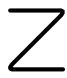
\includegraphics[keepaspectratio]{images/part001_11d71cd9.jpg}}

Remarks. 1) There can be infinitely many integrals of a differential equation (1) taking the same value at a given point. For example, the scalar differential equation \(x' = 2\sqrt{|x|}\) has all the functions defined by

\[
\begin{array}{l l} u (t) = 0 & \text { for } \quad - \beta \leqslant t \leqslant \alpha \\ u (t) = - (t + \beta) ^ {2} & \text { for } \quad t \leqslant - \beta \\ u (t) = (t - \alpha) ^ {2} & \text { for } \quad t \geqslant \alpha \end{array}
\]

as integrals taking the value 0 at the point t = 0, for any positive numbers \(\alpha\) and \(\beta\) .

\begin{enumerate}
\def\labelenumi{\arabic{enumi})}
\setcounter{enumi}{1}
\tightlist
\item
  Peano's theorem no longer holds when \(\mathbf{E}\) is an arbitrary complete normed space of infinite dimension (IV, p.~204, exerc. 18).
\end{enumerate}

